 \documentclass{openetcs_report}
% Use the option "nocc" if the document is not licensed under Creative Commons
%\documentclass[nocc]{template/openetcs_article}
\usepackage{todonotes}
\usepackage{appendix}
\usepackage{lipsum,url}
\usepackage{pdfpages}
%\usepackage{bibtopic} % Multibib
\usepackage{booktabs}
\usepackage{hyperref}

\usepackage[section,                 % add the glossary to the table of content 
            description,             % acronyms have a user-supplied description,
            style=superheaderborder, % table style
            nonumberlist             % no page number
]{glossaries}
\hypersetup{
linkbordercolor 	={1 1 1}}

%===========================
% Graphicpath
%===========================
\graphicspath{{./template/}{.}{./images/}}

%===========================
% Abbreviation file
%===========================
% \renewcommand*{\glossaryname}{List of Terms}
% \makeglossaries
% \loadglsentries{wp7_glossary} 
%===========================
%===========================
% Todo note margin
%===========================
\setlength{\marginparwidth}{7em}
\let\oldmarginpar\marginpar
\renewcommand\marginpar[1]{\-\oldmarginpar[\raggedleft\footnotesize #1]%
{\raggedright\footnotesize #1}}
%===========================

\begin{document}

\frontmatter
\project{openETCS}

%Please do not change anything above this line
%============================
% The document metadata is defined below

%assign a report number here
\reportnum{OETCS/WP7/D7.3}

%define your workpackage here
\wp{Work-Package 7: ``Toolchain''}

%set a title here
\title{Toolchain Qualification Process Description}

%set a subtitle here
%\subtitle{}

%set the date of the report here
\date{January 2014}

%define a list of authors and their affiliation here

\author{Cecile Braunstein \and Jan Peleska}

\affiliation{University Bremen}

\author{Stefan Rieger}

\affiliation{TWT GmbH Science \& Innovation\\
Ernsthaldenstraße 17\\
70565 Stuttgart\\
Germany
}


% define the coverart
\coverart[width=350pt]{openETCS_EUPL}

%define the type of report
\reporttype{Qualification process description}


\begin{abstract}
%define an abstract here
This document presents  different ideas of a toolchain
qualification. It describes a process  for the openETCS toolchain
qualification.  
\end{abstract}


%=============================
%Do not change the next three lines
\maketitle
\tableofcontents
%\listoffiguresandtables

\newpage
%=============================

% The actual document starts below this line
%=============================
%Start here
%=============================
% Document Managment
%=============================
\chapter{Document Information}

\begin{tabular}{|p{4.4cm}|p{8.7cm}|}
\hline
\multicolumn{2}{|c|}{Document information} \\
\hline
Work Package &  WP7  \\
Deliverable ID or doc. ref. & D7.3\\
\hline
Document title & Toolchain Qualification Process Description \\
Document version & 01.04 \\
Document authors (org.)  & Cécile Braunstein and Jan Peleska (Uni.Bremen) \\
\hline
\end{tabular}

\begin{tabular}{|p{4.4cm}|p{8.7cm}|}
\hline
\multicolumn{2}{|c|}{Review information} \\
\hline
Last version reviewed & 01.00 \\
\hline
Main reviewers &  Marielle Petit-Doche, Michael JastramJ, Jaime Paniagua\\
\hline
\end{tabular}

\begin{tabular}{|p{2.2cm}|p{4cm}|p{4cm}|p{2cm}|}
\hline
\multicolumn{4}{|c|}{Approbation} \\
\hline
  &  Name & Role & Date   \\
\hline  
Written by    &  Cécile Braunstein & WP7-T7.3 Sub-Task  & 12.01.2014 \\
&  & Leader&\\
\hline
Approved by &  &   &  \\
\hline
\end{tabular}

\begin{tabular}{|p{2.2cm}|p{2cm}|p{3cm}|p{5cm}|}
\hline
\multicolumn{4}{|c|}{Document evolution} \\
\hline
Version &  Date & Author(s) & Justification  \\
\hline  
00.00 & 12.01.2014 & C. Braunstein  &  Document creation  \\
01.00 & 19.01.2014 & C. Braunstein  &  Jan Peleska suggestions \\
01.01 & 28.01.2014 & M. Jastram  &  Review \\
01.02 & 28.01.2014 &  C. Braunstein &  Change from MPD, MJ JP suggestions \\
01.03 & 08.05.2014 &  S. Rieger &  Provide first draft of a tool qualification example \\
01.04 & 08.05.2014 &  S. Rieger &  Provide  another  tool qualification example \\


\hline  
\end{tabular}
\newpage
%==========================================


%------ List of terms and definition ----------------
%\printglossary
%==========================================
\mainmatter
%----------------------







\chapter{Introduction to Toolchain Qualification}
\label{chap-1}
\section{Tool Qualification}
\label{sec-1-1}


The CENELEC EN 50128 standard \cite{standard_railway_2011} defines the tool
qualification as follows:\\
{\it ``The objective is to provide evidence that potential
failures of tools do not adversely affect the integrated tool-set output in a
safety related manner that is undetected by technical and/or organizational
measures outside the tool. To this end, software tools are categorized into
three classes namely, T1, T2 \& T3 respectively.''}

We recall here the different class definitions:
\begin{itemize}
\item Tool class T1: No generated output can be used directly or indirectly to the
  executable code;
\item Tool class T2: Verification tools, the tool may fail to detect errors or
  defects;
\item Tool class T3: Generated output directly or indirectly  as part of the
  executable code.
\end{itemize}
The deliverable D2.2 \cite{pokam_report_2013} summarizes the requirements for the
tool needed by the different tool classes. The report highlights that the
effort differs depending on the tool class. Furthermore, for
the most critical class T3,  the evidence should be provided that the output is
conform to the specification or that \emph{any failure in the output
  are detected}. 

The standard defined how to classify each tool individually (see
\cite{nielsen_efficient_2012,huang_test_2013} as an example).  But dealing with a tool
chain, integrated within a tool platform, implies extra effort to
ensure that the tool integration does not introduce new errors. For
example mechanism such as artifacts versioning, time-stamping
operations, etc ... should also be considered when qualifying the tool
chain.

In summary, the effort of qualification depends on the tool class and the tool
error detection capabilities. To reduce the cost of the toolchain qualification
and regarding the fact that our development imply regular releases, a systematic
toolchain analysis approach has to be defined.
 
\section{Toolchain Qualification State of the Art}
\label{sec-1-2}
Some recent works have been done in the field of toolchain
qualification from a variety of projects. The next section summarizes
the most significant ones.

\subsection{Slotosh and al. (project RECOMP)}
\label{sec-1-2.1}

 \cite{slotosch_model-based_2012} describes a model-based approach to tool
 qualification to comply with DO-330 and integration into the Eclipse
 development environment. The authors claim that the benefits of their
 method  are the following:

\begin{description}
\item[Clarity:] remove ambiguities;
\item[Re-usability and Transparency:] check for reuse in different toolchain;
\item[Completeness:] the model covers all parts of the  development
  process and tis traceable;
\item[Automation:] Some part of the process may be automated.
\end{description}

Their method is explained in detail in \cite{slotosch_iso_2012}: the
toolchain analysis is based on a domain specific toolchain model
they have defined. This model is used to represent the toolchain
structure as well as the tool confidence.  Their goal is to deduce the
tool confidence level and to expose specific qualification
requirements, furthermore, their idea is not only to check tool by
tool but to have a more holistic approach and makes use of
rearrangement and/or the extension of the toolchain to avoid the
certification of all tools. This allows them to reduce the
qualification effort by focusing only on the critical tools and make
use of already available information.  Moreover, some inconsistencies
check such as, missing description, unused artifacts ..., may be
automatically done by using the toolchain model. Finally, they
provide support to automatize the document production.

\cite{wildmoser_determining_2012} apply their tool and methods an
industrial use case to determine the potential errors in the tool-chain.

\subsection{Asplund and al. (projects iFEST, MBAT)}
\label{sec-1-2.2}

The authors investigate the question if there exists part of the environment related to tool
integration that may fall outside the tool qualification defined by the a norm
(ISO 26262 here \cite{asplund_qualifying_2012}). And if so, how tool integration
is affected by ensuring functional safety. One conclusion is that the tool
integration may lead to increase the qualification effort.

They also state that the standards (EN 50128, DO-178C and ISO26262)
are not sufficient to check safety of a toolchain, but some part of a
toolchain may be taken into account to mitigate the qualification
effort. 
They highlight 9 safety issues caused by tool integration that also
allow to be more exact when identifying software that have to be
qualified for certification purpose. 

They advocate that to deal with the qualification of tool integration
within a toolchain a system approach should be taken, we should not
thing about individual tools anymore.  Their proposed method is a ``System
Approach'' for toolchain qualification following these steps:

\begin{enumerate}
\item Pre-Qualification of development tool (requirements tools,design
  tools ...): provided by the vendors.
\item Pre-qualification at the tool-chain level: based on step 1 and
  reference work-flows, defined where are the safety critical part.
\item Qualification of the tool-chain: check differences of step 2 and
  the actual deployed toolchain.
\item Qualification at the tool level: based on the actual environment
  when deploying the toolchain.
\end{enumerate}
This approach leads them to separate the parts required to software tool
qualification and to identify safety issues related to tool integration.

In \cite{asplund_towards_2012}, they explore the step 2): identifying
the required safety goals due to tool integration and obtain a
description of a reference work-flow and tool-chain with annotation
about the mitigating effort.  They proposes to use the TIL language, a
domain specific language for toolchain model.  The model of the tool
chain is used to perform a risk analysis and to annotate parts
that need mitigating effort for the safety issues due to tool
integration. 

\subsection{Biehl and al. (projects CESAR, iFEST, MBAT)}
\label{sec-1-2.3}

Biehl proposed a Domain Specific Language named TIL for Generating Tool Integration
Solutions \cite{biehl_matthias_domain_2011}.  A toolchain is described in terms
of a number of ``Tool Adapters'' and the relation between them.
\begin{itemize}
\item ToolAdapters: exposes data and functionality of a tool
\item Channels
  \begin{itemize}
  \item ControlChannels describe service calls
  \item DataChannel describe data exchanges
  \item TraceChannel  describe creation of a trace links
  \end{itemize}

\item Sequencer: describe sequential control flow (sequence of services)
\item User:  describe and limit the possible interaction
\item Repository:  provide storage and version Management of tool data
\end{itemize}
This DSL allows early analysis of the toolchain.
It may generate part of tool adapter code based on the source and target
meta-model.

More recently, Biehl and al.  define a standard language for modeling
development process defines by OMG 2008. The language has been used in
\cite{biehl_constructing_2012,biehl_early_2012} together with the TIL
language to tailor a toolchain following a process model. The goal is
to be able to model both the development process and the set of tools
used.  A process is defined as follows:
\begin{itemize}
\item Process: several Activities
\item Activity: set of linked Tasks, WorkProducts, Roles
\item A Role can perform a Task
\item A WorkProduct can be anaged by a Tool
\item A Task can use a Tool
\end{itemize}
Using together the process development language  and the toolchain
language, in \cite{biehl_early_2012}, the authors  measure the alignment of a toolchain
with a product development process. The method proceeds as follows:
\begin{enumerate}
\item Inputs:
  \begin{itemize}
  \item formalized description of the toolchain design
  \item description of the process including the set of tools and their capabilities
  \end{itemize}
\item Initial verification graph
\item Automatic mapping links to the verification graph (acc. to mapping rules)
\item Apply alignment rule on the verification graph
\item Apply metrics to determine the degree of alignment btw the tool-chain and the
   process
\end{enumerate}
The metrics and the misalignment list provide feedback to refine the tool-chain
design.



%%% Local Variables: 
%%% mode: latex
%%% TeX-master: "oetcs_qualification_process"
%%% End: 




\chapter{OpenETCS Toolchain Qualification Process}
\label{chap-2}
\section{Toolchain Analysis}
\label{sec:toolchain-analysis}

All the methods mentioned above start with a complete definition of the toolchain. In OpenETCS, the development of the toolchain follows an \emph{agile} approach.
Hence, for each (major) release we have to deal with an incomplete tool
chain. In addition to the methods of the previous section,  we need a qualification
process that can adapt to the development speed, deal with an incomplete toolchain
and can re-use qualification information.

Moreover, as stated by Asplund et al., the toolchain itself may
provide some mechanism that may reduce the tool qualification effort
\cite{asplund_towards_2012,asplund_qualifying_2012}. They are
descibred as a set of safety goals that the tool chain should ensure.
 In our context, most of the
tool integration effort is made by integrating tools into a tool
platform.  According to Asplund et al., the tool platform should
ensure the following safety-goals that will avoid some extra tool qualification:
\begin{itemize}
\item Coherent time stamp information: common time stamps on development artifacts.
\item Notification: the user should be notified when artifacts changed.
\item Data integrity:  avoid use of obsolete artifacts, the data used reflects the
  current state.
\item Data mining: all data used by safety analysis should be available and be
  verifiable.
\end{itemize}

\begin{figure}
\begin{center}
\begin{tikzpicture}[->, >=stealth,node distance=1.5cm, auto]
\tikzstyle{decision} = [diamond, draw, fill=blue!20, align=center]
\tikzstyle{block} = [rectangle, draw, fill=blue!20, align=center, rounded corners]
	\node [block] (n1) {Features Analysis};
	\node [block, below of=n1] (n2) {Toolchain Platform Analysis};
	\node [block, below of=n2] (n3) {Design Qualification Plan};
	\node [below of=n3] (sub3) {};
	\node [left of=sub3, node distance=4cm] (label1) {Toolchain \& Platform Development};
	\node [block, below of=label1, node distance=1cm] (n4) {Functional Specification};
	\node [block, below of=n4] (n5) {Code Development};
	\node [block, below of=n5] (n6) {Code Review};
	\node [block, below of=n6] (n7) {Testing};
	\node [block, right of=sub3, node distance=4cm] (n8) {Tools Evaluation};

	\node [below of=n8,align=center, node distance=2cm] (tq1) {Individual Tool Qualification\\(to be followed for each tool)};

	\node [block, below of=tq1, node distance=1.5cm] (tq2) {Operational\\Qualification};
	\node [block, left of=tq2, node distance=2.5cm] (tq3) {Installation\\Qualification};
	\node [block, right of=tq2, node distance=2.5cm] (tq4) {Performance\\Qualification};
	\begin{scope}[on background layer]
		\node [block, fit=(tq1) (tq2) (tq3) (tq4)] (n9) {};
		\node [block, fit=(label1) (n4) (n5) (n6) (n7)] (n10) {};
	\end{scope}
	\node [block, below of=n3, node distance=9cm] (n11) {Tool \& Platform Integration};
	\node [block, below of=n11] (n12) {Toolchain Installation Qualification};
	\node [block, below of=n12] (n13) {Toolchain Operational Qualification};
	\node [block, below of=n13] (n14) {Toolchain Performance Qualification};
	\node [block, below of=n14] (n15) {Maintenance};

	\draw[->] (n1) -- (n2);
	\draw[->] (n2) -- (n3);
	\draw[->] (n3) -- (n10);
	\draw[->] (n3) -- (n8);
	\draw[->] (n8) -- (n9);
	\draw[->] (n4) -- (n5);
	\draw[->] (n5) -- (n6);
	\draw[->] (n6) -- (n7);
	\draw[->] (n9) -- (n11);
	\draw[->] (n10) -- (n11);
	\draw[->] (n11) -- (n12);
	\draw[->] (n12) -- (n13);
	\draw[->] (n13) -- (n14);
	\draw[->] (n14) -- (n15);
\end{tikzpicture}
\end{center}
\caption{Qualification process as proposed by Izaskun de la Torre}
\label{fig:qualification_process_idelatorre}
\end{figure}

\begin{figure}
\begin{center}
\scalebox{0.9}{
\begin{tikzpicture}[->, >=stealth,node distance=1.5cm, auto]
\tikzstyle{decision} = [diamond, draw, fill=blue!20, align=center, font=\footnotesize]
\tikzstyle{block} = [rectangle, draw, fill=blue!20, align=center, rounded corners]
	\node [block] (n1) {Features Analysis};
	\node [block, below of=n1] (n2) {Toolchain Platform Analysis};
	\node [below of=n2,align=center] (l1) {Individual Tool Qualification (to be followed for each tool)};
	\node [block, below of=l1, node distance=1cm] (n3) {Define Process \& Usage Context};
	\node [block, below of=n3] (n4) {Tool Classification};
	\node [decision, below of=n4, anchor=north] (d1) {Tool is\\prequalified};
	\node [below of=d1, node distance = 3cm] (subd1) {};
	\node [block, left of=subd1, node distance=4.5cm] (n5) {Check conformance\\with defined process\\and usage context};
	\node [decision, right of=subd1, node distance=4.5cm] (d2) {Qualification\\by third party\\possible};
	\node [block, below of=d2, node distance=3cm] (n6) {Provide process and usage context\\for third party qualification};
	\node [decision, below of=d1, node distance= 3cm] (d4) {Conformance?};
	\node [decision, below of=d4, node distance=3cm] (d3) {Tool is\\open source};
	\node [below of=d3, node distance = 2.53cm] (subd3) {};
	\node [block, fill=red!20, right of=subd3, node distance=2.5cm] (n7) {Qualification impossible\\(except ``proven in use'')};
	\node [block, left of=subd3, node distance=2.5cm] (n8) {Operational Qualification\\by Tool Chain Integrator};
	\node [block, below of=d4, node distance=8cm] (n9) {Tool-to-Platform Integration Qualification};
	\begin{scope}[on background layer]
		\node [block, fill=black!10, fit=(l1) (n3) (n4) (d1) (n5) (d2) (n6) (n9)] (individual_quali) {};
	\end{scope}
	\node [block, below of=n9] (n10) {Toolchain Installation Qualification};
	\node [block, below of=n10] (n11) {Toolchain Operational Qualification};
	\node [block, below of=n11] (n12) {Toolchain Performance Qualification};

	\draw[->] (n1) -- (n2);
	\draw[->] (n2) -- (individual_quali);
	\draw[->] (n3) -- (n4);
	\draw[->] (n4) -- (d1);
	\draw[->] (d1) -- node [near start] {yes} (n5);
	\draw[->] (d1) -- node [near start] {no} (d2);
	\draw[->] (d2) -- node [near start] {yes} (n6);
	\draw[->] (d2) -- node [near start] {no} (d3);
	\draw[->] (d3) -- node [near start] {no} (n7);
	\draw[->] (d3) -- node [near start] {yes} (n8);
	\draw[->] (n5) -- (d4);
	\draw[->] (d4) -- node [near start] {no} (d2);
	\draw[->] (n8) -- (n9);
	\draw[->, out=190, in=180] (d4) to node [near start] {yes} (n9);
	\draw[->, out=-50, in=0] (n6) to (n9);
	\draw[->] (individual_quali) -- (n10);
	\draw[->] (n10) -- (n11);
	\draw[->] (n11) -- (n12);
\end{tikzpicture}}
\end{center}
\caption{Proposed adaptation by Stefan Rieger (among other changes, the TC development branch was removed as this work is not part of qualification itself)}
\label{fig:qualification_process_srieger}
\end{figure}

\section{Scenario-based Qualification of Individual Tools}
\label{sec:scenario-based-tool-quali}

Qualifying a toolchain always requires the qualification of the individual tools it is comprised of. The effort required depends on the type and license of the tool to be qualified. To this end in the following we have identified a number of different scenarios that are of relevance in the context of the openETCS project as depicted in Figure~\ref{fig:tool-qualification-scenarios}.

\begin{figure}
\begin{center}
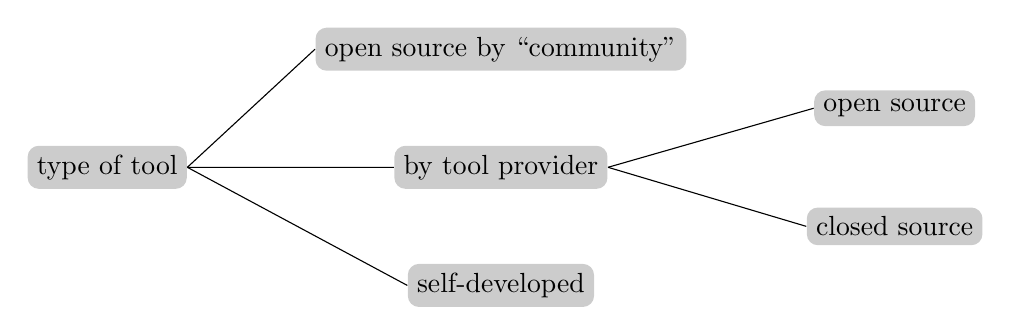
\begin{tikzpicture}[parent anchor=east,child anchor=west,grow=east, edge from parent, level distance=5cm]
	\tikzstyle{every node}=[fill=black!20,rounded corners]
	\node {type of tool}
		child { node {self-developed} }		
		child { node {by tool provider}
			child { node {closed source} }
			child { node {open source} }
		}
		child { node {open source by ``community''} };
\end{tikzpicture}
\end{center}
\caption{Scenarios to consider when qualifying individual tools}
\label{fig:tool-qualification-scenarios}
\end{figure}

In the following considerations for the individual scenarios are described.

\subsection{Self-developed Tool}

For a self-developed tool the project needs to provide the means for qualification and quality assurance. As the tool has not been employed in productive use by others the ``proven in use'' argument \textcolor{red}{[Remark: It needs to be checked whether this argument actually applies to EN 50128]} does not apply.

\subsection{Tool Provided by a Tool Provider}

For tools provided by a third party we must distinguish again two cases:

\paragraph{The tool is provided as closed source tool}

If the tool is not pre-qualified by the tool provider the options are limited. If the tool provider is not willing or unable to provide the means for qualification, the qualification of the tool will be almost impossible. One exception might be if the tool is already in use on a broad scale in industry and is generally regarded as reliable for the intended purpose. Also the tool class must be considered here.

\paragraph{The tool is provided as open source}

In this case it would be possible to adapt the tool and analyse it to enable qualification. However, this involves a huge amount of effort which is best done by the tool provider who as a better insight into the tool's internal workings. Also a third party who has already experience with the tool or is a specialist with regards to qualifying safety-critical tools could be entrusted with the qualification task.

\subsection{Open Source Tool Provided by the ``Community''}

If no tool provider can be identified but the tool is developed by the community and distributed under an open source license, the tool qualification has to be conducted by the project. However, many open source tools have a large development and expert community which can certainly be of help. In addition, the ``proven in use'' argument could possibly be applied (e.g., for tools like GCC).

\section{Incremental Tasks for toolchain qualification}
The qualification of the toolchain shall follow an incremental process adding the next tool to the previously qualified tool chain. The process will continue until the last qualified tool is integrated and the complete toolchain is qualified. The botton-up approach will be applied. As a result, the errors related to intertool interface should be easier to pinpoint.

After the individual tools are qualified, their integrations into the toolchain are planned. As part of the integration planning, the team will analize the dependencies of the different tools to minimize the effects of unavoidable dependencies. 

When each iteration is released, a new qualification process should be conducted following the previously commented phases:
\begin{itemize}
\item Installation qualification: Installation should verify that the toolchain is properly installed. It does not verify that the toochain conforms to the functional and performance specification. This is done later in the OQ phase..  to verify correct software installation and to document all computer hardware, software and configuration settings as the initial baseline configuration.
\item Operational qualification: should demonstrate that the toolchain will function according to its operational specification in the selected environment. The tests should be performed to verify that the toolchain meets the specifications, requirements in the specific environment.
\item Performance qualification: should demonstrate that the toolchain consistently performs according to the specifications defined by the openETCS project, and is appropriate for the intended use. Important for consistent openETCS toolchain performance are regular preventive maintenance, making changes to the toolchain in a controlled manner and regular testing.

The toolchain should be well maintained to ensure proper ongoing performance. Procedures should be in place for regular preventive maintenance of it to detect and fix problems before they can have a negative impact.
\end{itemize}

During the toolchain qualification it will be iterative tasks where users repeat a set of actions over and over again so it would be necessary to evaluate these type of tasks and try to automate a subset of them to minimize the execution time.


\section{Model-based Tool Qualification}
\label{sec:model-based-tool-quali}

This section describes a proposal on how to setup the operational qualification of individual tools. This step of the qualification process (cf. Figure~\ref{fig:qualification_process_srieger}) is required for any tool that is not pre-qualified. With respect to the scenarios described in Section~\ref{sec:scenario-based-tool-quali} it applies to self-developed and third party open source tools. In the case of closed source tools it is not possible to follow this process as the internal workings of the tools are hidden.

We propose setting up the operational tool qualification based on the approach by Slotosch et al. which has been briefly sketched in Section~\ref{sec:slotosh-approach}. In particular we will focus on the artifacts and documentation necessary to conduct the qualification steps. Figure~\ref{fig:qualification-models-linkage} shows the different parts of the qualification model according to \cite{slotosch_model-based_2012}. Some links are not directly evident in the paper but have been added where reasonable. In the context of openETCS the ``Quality Assurance'' part mentioned in \cite{slotosch_model-based_2012} is covered by using the GitHub issue tracker and is thus not explicitly considered in the following.

\begin{figure}
\begin{center}
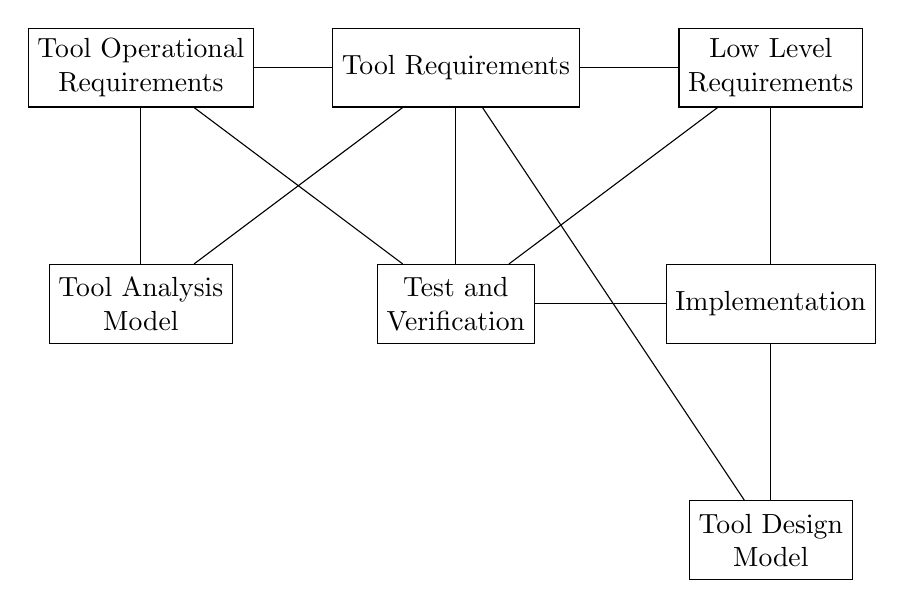
\begin{tikzpicture}
	\tikzstyle{block} = [rectangle, draw, align=center, minimum width=2cm, minimum height=1cm]
	\node[block] (n1) at (0,0) {Tool Operational\\ Requirements};
	\node[block] (n2) at (4,0) {Tool Requirements};
	\node[block] (n3) at (8,0) {Low Level\\Requirements};
	\node[block] (n4) at (0,-3) {Tool Analysis\\Model};
	\node[block] (n5) at (8,-6) {Tool Design\\Model};
	\node[block] (n6) at (8,-3) {Implementation};
	\node[block] (n8) at (4,-3) {Test and\\Verification};
	\draw (n4) -- (n1);
	\draw (n4) -- (n2);
	\draw (n1) -- (n2);
	\draw (n2) -- (n3);
	\draw (n3) -- (n6);
	\draw (n2) -- (n5);
	\draw (n5) -- (n6);
	\draw (n8) -- (n1);
	\draw (n8) -- (n2);
	\draw (n8) -- (n3);
	\draw (n8) -- (n6);
\end{tikzpicture}
\end{center}
\caption{Parts of the qualification model and their linkage according to \cite{slotosch_model-based_2012}}
\label{fig:qualification-models-linkage}
\end{figure}

The two SysML block diagrams depicted in Figures~\ref{fig:requirements_model} and \ref{fig:tool_analysis_model} depict qualification metamodels for openETCS derived from \cite{slotosch_model-based_2012}. They need to be instantiated for each individual tool.

\begin{figure}
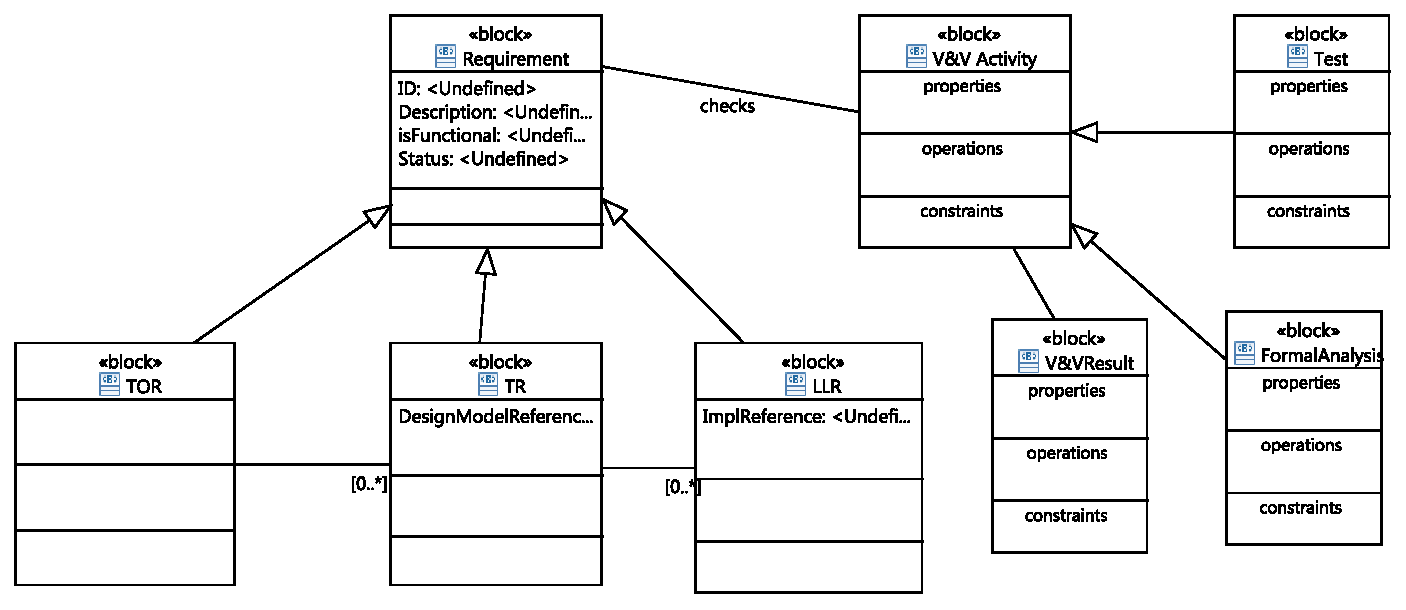
\includegraphics[width=\textwidth]{RequirementsModel.pdf}
\caption{Requirements meta model for qualification}
\label{fig:requirements_model}
\end{figure}

\begin{figure}
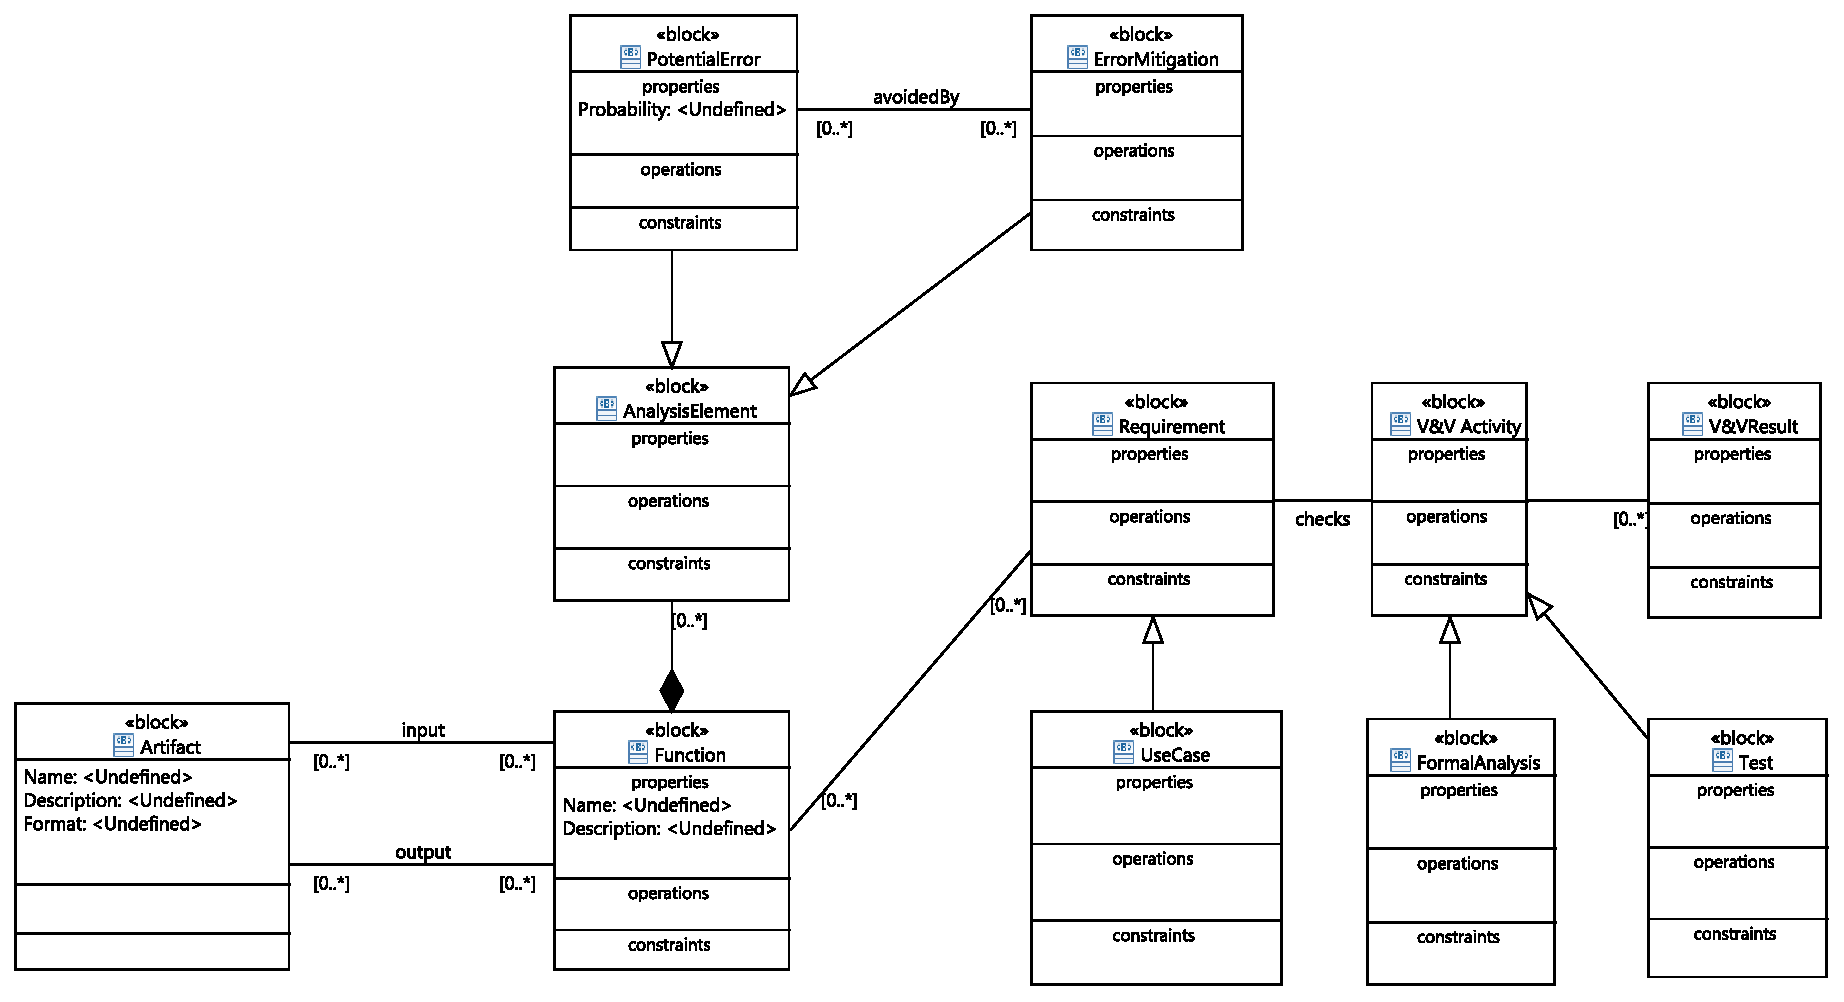
\includegraphics[width=\textwidth]{ToolAnalysisModel.pdf}
\caption{Tool analysis meta model for qualification}
\label{fig:tool_analysis_model}
\end{figure}

\subsection{Requirements Model}

The requirements are represented on three different levels of abstraction interlinked with each other.

\paragraph{Tool Operational Requirements (TORs)}
The tool operational requirements are derived from both, the safety standard applicable for openETCS, CENELEC EN 50128, and the operating environment of the tool based on the use cases. They determine the tool confidence level and the tool classification. Each tool operational requirement can be refined by any number of tool requirements. 

\paragraph{Tool Requirements (TRs)}
Tool requirements break down the high level TORs to architectural / design level. Thus, they are interlinked with the design model. Each tool requirement may be linked with any number of low level requirements. 

\paragraph{Low Level Requirements (LLRs)}
Requirements at code level that are linked directly with the code.

\subsection{Tool Analysis Model}
The tool analysis model is used to analyse the functions of the tool and potential errors and mitigations. According to \cite{slotosch_model-based_2012} it can be used to automatically derive tool qualification levels (at least for the automotive and aerospace safety standards). In the context of openETCS it should be used as a means to document the tool functions, their assignment to requirements (TORs and TRs) and the artifacts that are used/processed by them (inputs and outputs).

\subsection{Tool Design Model}
The tool design model shall represent the architecture of the tool to be qualified. Tool requirements shall be allocated to design elements which in turn shall be traceable to the implementation (e.g., references to specific functions, classes or model elements in the context of SCADE modelling). In the context of openETCS the tool design model is built using SysML with the Papyrus tool.

\subsection{Implementation}
In openETCS the implementation is mainly consisting of a SCADE model that should be structured in a clear way, e.g., to allow referencing of implemented functions.

\subsection{Test and Verification}


\section{OpenETCS Toolchain Qualification Process}
\label{sec:toolchain-qualification-process}

The OpenETCS tool chain  will be defined by the set of its features and
a guideline describing how to correctly use it.
A SysML block diagram describes the tool chain architecture at a certain point in time as shown in
Figure \ref{fig:overview}. 
\begin{figure}[htbp]
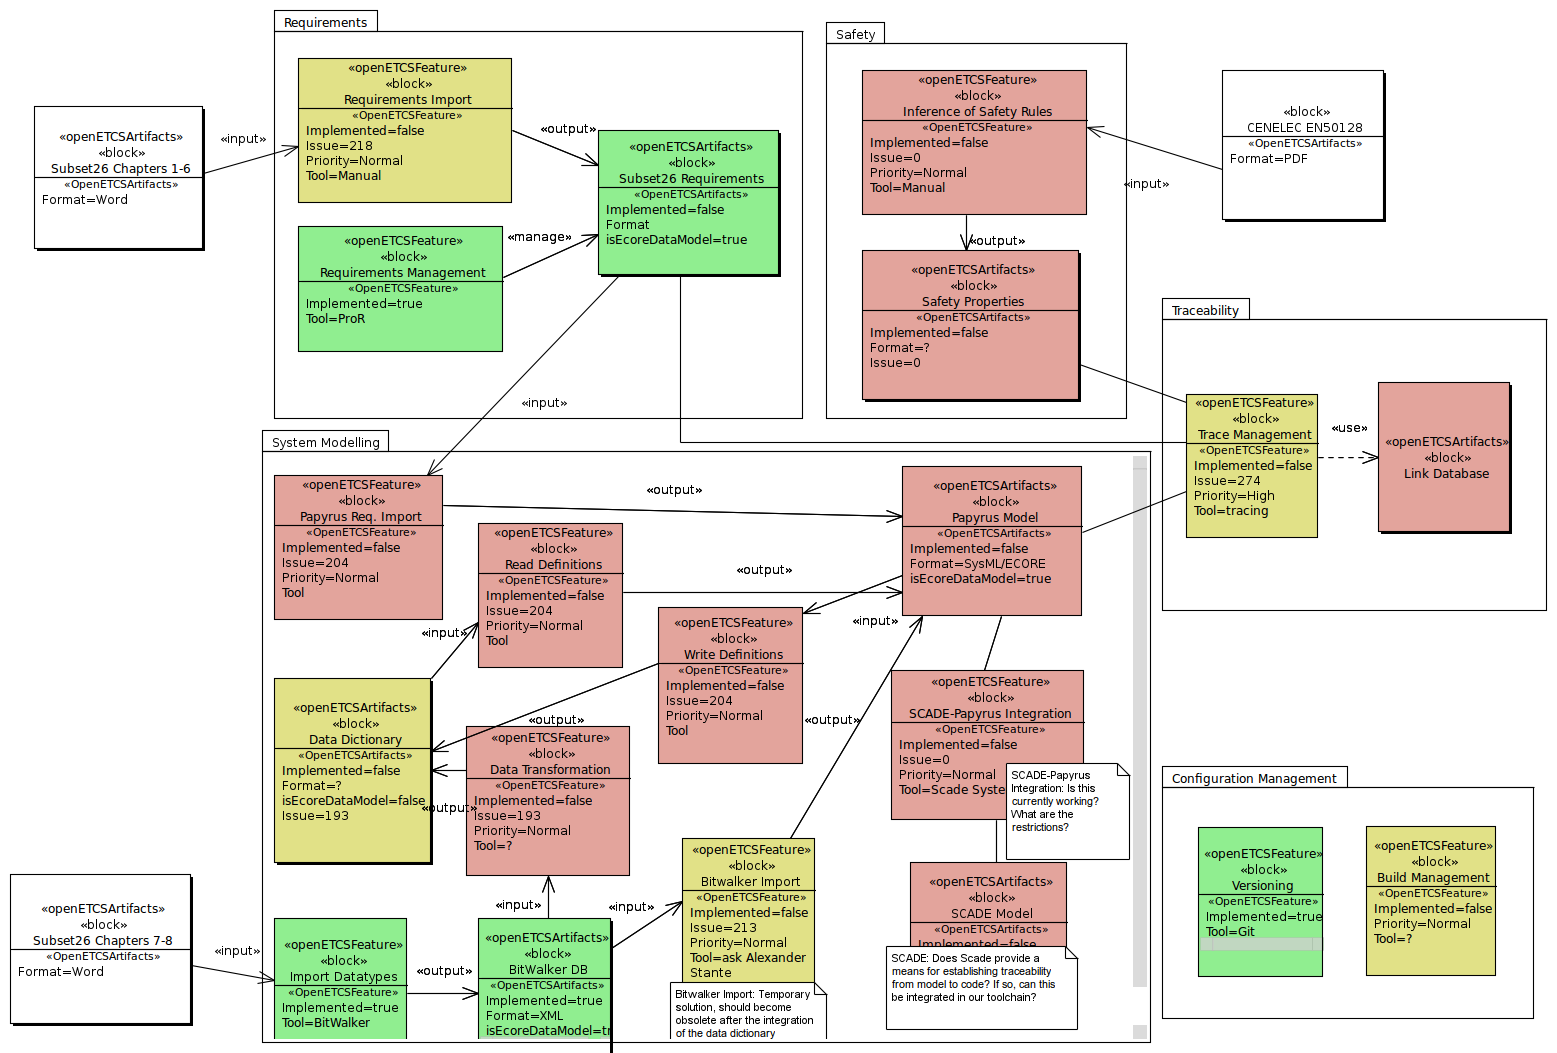
\includegraphics[width=\textwidth]{ToolChainmodel}
\caption{\label{fig:overview} Tool Chain overview (20.02.14) -- \\
  Green Block: Implemented \\
  Yellow Block: Work in Progress \\
  Red Block: Not started \\
  White Block: External Artifacts} 
\end{figure}

This block diagram is intended to grow according to new feature requests and the
needs of openETCS participants.  This diagram will be kept updated
as a reference of our tool chain. In any case, the complete information
regarding the feature availabilities  may be found in the Eclipse product
definition.

Each feature of the toolchain is a block with the profile ``openETCSFeature''
and  each artifact is block with the profile ``openETCSArtifact''.  Each
feature realizes at least one use case and may be implemented by one or more tools.
Note that in the tool platform features  may also be
implemented as plug-ins. The diagram also imposes a (partial) order
on the tasks. While some may be done in parallel, many tasks are dependent on others.
Currently, the diagram neither highlights the use of the tools, nor the order of actions
to be performed. This diagram should be completed by guidelines on
how to use the tool chain and/or an activity diagram.

To mitigate the qualification process, we will first consider more
than one feature at a time considering that errors from a tool A may
be detected by a Tool B in the next step of the tool chain process.
Furthermore, the toolchain is a collection
of features and not only tools. This differs from Asplund and al. in the sense that
some of the tool integration mechanisms that automate transformation of data, represent features
 and are thus not out of the scope of the qualification.

Due to our development process, a ``pre-qualification'' of tools should be made
when integrating a tool.

\todo[inline]{This high-level list should be detailed.}
\paragraph{Tool Integration Process for Qualification}

\begin{itemize}
\item Define name and version
\item Describe use cases
\item Provide justification of the tool within the tool chain
\item Provide input/output artifacts format (associated with the
  version)
\item Integrate the tool in the SysML model
\item Provide tool manual and other available documentation (associated with the version)
\item Link with an issue tracker
\end{itemize}

One possible implementation is to represent all these in formations
directly in the SysML model.

\todo[inline]{This high-level list should be detailed.  What I would expect: Which artefacts exist; How they are connected; When artefacts have to be re-validated (e.g. due to changes); What roles exist; who is responsible for what; etc.}
\paragraph{The Qualification Process}

\begin{enumerate}
\item Feature Analysis
  \begin{itemize}
  \item This step should assign a class to each feature based on the use cases.
  \item Define the potential errors
  \item Identify counter measure and/or error detection
  \item For T3 tools 2 alternatives:  certified compiler/generator or
    object code checker and/or exhaustive tester
  \end{itemize}
\item Tool platform  analysis 
  \begin{itemize}
  \item Provide evidence that the safety-goals mentioned in the
    previous sub-section are fulfilled\textcolor{red}{[The identification of safety goals is missing in step 1]}
  \end{itemize}
\item Toolchain Analysis
  \begin{itemize}
  \item Defines the work-flow
  \item Identify the ``hot spots'' of the toolchain
  \item Rearrange the toolchain if possible
  \item Find new measures when needed with combining tools (redundancy with orthogonal
    codes \ldots{})
  \end{itemize}
\item Toolchain qualification verification 
  \begin{itemize}
  \item Check consistency of tool version with  manuals and other
    provided feature information
  \item Generate table to  check if all possible errors has a
    detection or a correction mechanism
\item Generate the qualification report
  \end{itemize}

\end{enumerate}









\chapter{Example - Considerations for two openETCS Features}
\label{chap-example}
 \section{Bitwalker}
\begin{longtable}{lp{0.7\textwidth}}
&\textbf{Bitwalker - Import of Data Types and Variables}\\
Input&Subset-026-7, Subset-026-8, MS Word Format\\
Output&Database (XML) representing data types, variables and messages\\
Tool Class&T3\\
          &The resulting definitions are direct input to the model and thus any fault may be propagated down to the code level\\
Safety Integrity Level&? \textcolor{red}{[Currently I do not have the EN 50128 standard available]}\\
Potential errors&The following list is not exhaustive and shall just give some ideas. The feature implementor has to provide more detail.
                                \begin{itemize}
                                  \item Variable / message / type not detected or missing in output\newline
                                       Mitigation: This error can possibly be detected avoided as the modelling process is manual. Required in- or output described in the
                                                   SRS can be added manually if missing.
                                  \item Variable or message have wrong type (*)\newline
                                       This is a very dangerous error, especially in the case of different precision integers or floats. The error may
                                       remain unnoticed and be propagated to the code leading to potentially fatal malfunctions. A mitigation is only possible by
                                       manual recheck (which would make an automatic conversion obsolete) of extensive/exhaustive testing or verification of the tool 
                                       implementing the feature. However the inconsistent nature of the input document (Word) could prevent this.
                                  \item Missing fields in record / message\newline
                                       Mitigation: Can be detected if the functionality of the field is described in the functional description.
                                  \item Wrong naming of variable / message / type (**)\newline
                                       Mitigation: Potentially dangerous if names of variables (of compatible type) are mixed up. The risk is the same as for wrong typing.
                                  \item ...
                                \end{itemize}
                               \\
Providing evidence&It will be necessary to provide evidence that critical errors such as (*) and (**) can be detected or are not present in the tool. 
                   Exhaustive verification will be difficult due to the unreliable structure of the input document. The result must be correct
                   also for ill-formed documents. A solution would be to let ERA acknowledge the converted XML database as a formal document. In this case the tool can be classified T1.

\end{longtable}

\section{RT-tester qualification example}
\subsection{Tool identification}
\begin{description}
\item[Name:]  RTT-MBT - Model-Based Test Generator
\item[Version :]  8.9-4.1.2
\end{description}
\subsection{Tool Justification}
The use of RT-tester allow to tests the C code produced by SCADE,
B. It automatically generates tests for the following coverage
criteria:  basic control state coverage, transition coverage, MC/DC
coverage and requirement coverage.

\subsection{Use cases}
\paragraph{Tool classification}
\begin{description}
\item[Intended prurpose] Automated generation of test procedures for embedded HW/SW con-
trol systems
\item[Output] Test procedures to be executed in a test execution environment (both software
testing or hardware-in-the-loop testing environment) 
\item[Input] SysML test model (XMI format), test cases specification.
\item[Tool Class] T2: The tool may fail to detect errors or defects.
\end{description}
\paragraph{Use case description}
\begin{enumerate} 
\item {\bf Generation} Generate test cases, test data and test procedures from model.
\item {\bf Replay.} Replay test execution logs against the model.
\end{enumerate}

\paragraph{Potential Errors}
\begin{itemize}
\item Hazard 1: undetected SUT failures. The test oracles produced are
  incorrect and fail to observe a incorect behavior during test
  execution.
\item Hazard 2: undetected coverage failures. The test execution does
  not cover what it should. The test will pass but the result will not
  covered what it supposed to.
\end{itemize}




\bibliographystyle{plain}
\bibliography{D7.4}
\end{document}
